\documentclass[10pt,a4paper,twoside]{article}
\usepackage[english]{babel}
%laad de pakketten nodig om wiskunde weer te geven :
\usepackage{amsmath,amssymb,amsfonts,textcomp}
%laad de pakketten voor figuren :
\usepackage{graphicx}
\usepackage{float,flafter}
\usepackage{hyperref}
\usepackage{inputenc}
\usepackage{minted}
\usepackage{subcaption}

\setlength\paperwidth{20.999cm}\setlength\paperheight{29.699cm}\setlength\voffset{-1in}\setlength\hoffset{-1in}\setlength\topmargin{1.499cm}\setlength\headheight{12pt}\setlength\headsep{0cm}\setlength\footskip{1.131cm}\setlength\textheight{25cm}\setlength\oddsidemargin{2.499cm}\setlength\textwidth{15.999cm}

\newcommand{\sweepsize}{0.26}

\begin{document}
\begin{center}
\hrule

\vspace{.4cm}
{\bf {\Huge Computer Vision} \\ {\huge Lab Assigment Report} \\ {\Large Condensation Tracker}}
\vspace{.2cm}
\end{center}
{\bf Tuan Mate Nguyen}  (tunguyen@student.ethz.ch)
\hrule



\section{Implementation}
\subsection{Color histogram}
I only considered the bounding box of the ROI. This array is then flattened as
required by np.histogramdd(), which is a function for creating multidimensional
histograms. As we have 3 color channels and $hist\_bin$ number of bins for each
color dimension, the resulting histogram will have a size of $hist\_bin^3$.

The density parameter is set to false in order to obtain the number of sampes in
each bin. Then I explicitly normalized the bins by dividing the total number of
samples.

\subsection{$A$ matrix}
In case of no motion the state vector consist of only two elements,
corresponding to the $x$ and $y$ coordinates of the object. Since the prediction
model assumes no motion, the $A$ matrix will just be the identity matrix.

As for the constant velocity model, the state vector has 4 elements, the two
spatial coordinates and the velocities in the $x$ and $y$
directions. For the new coordinates we can write

\begin{eq}

\end{eq}

\subsection{Propagation}
\subsection{Observation}
\subsection{Estimation}
\subsection{Resampling}

\section{Experiments}
\subsection{Video 1}
\subsection{Video 2}
\subsection{Video 3}


% Python code
%\begin{minted}[mathescape,
%    linenos,
%    numbersep=5pt,
%    gobble=2,
%    frame=lines,
%    framesep=2mm,
%    firstnumber=26]{csharp}
%\end{minted}

% Image
%\begin{figure}[H]
%    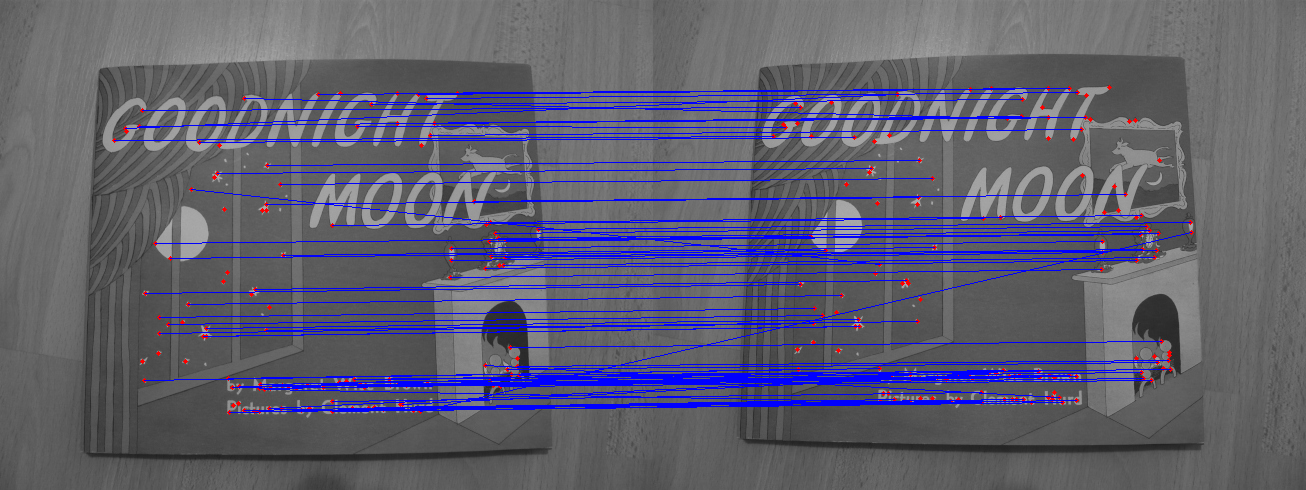
\includegraphics[width=\textwidth]{match_mutual.png}
%    \centering
%    \caption{Matching keypoints for mutual nearest neighbor matching}
%    \label{match_mutual}
%\end{figure}

\end{document}
